\documentclass[11pt]{article}
%%%%%%%%%%%%%%%%%%%%%%%%%%%%%%%%%%%%%%%%
\usepackage{amsmath}
\usepackage{verbatim}
\usepackage[usenames,dvipsnames]{color}
\usepackage{setspace}
\usepackage{lscape}
\usepackage{longtable}
\usepackage[top=1.25in,bottom=1.25in,left=1in,right=1in]{geometry}
\usepackage{graphicx}
\usepackage{epstopdf}
\usepackage[usenames,dvipsnames]{pstricks}
\usepackage{epsfig}
\usepackage{pstricks-add}
\usepackage{pst-node}
\usepackage{pst-plot}
\usepackage{fancyhdr}
\usepackage[absolute,showboxes]{textpos}
\usepackage{booktabs}
\usepackage{dcolumn}
\usepackage{arydshln}
\usepackage{natbib}
\usepackage{tabularx}

\setcounter{MaxMatrixCols}{10}
\newcolumntype{d}[1]{D{.}{.}{-2.#1}}
\newenvironment{proof}[1][Proof]{\noindent\textbf{#1.} }{\ \rule{0.5em}{0.5em}}
\setlength{\columnsep}{.2in}
\psset{unit=1cm}

\def\sym#1{\ifmmode^{#1}\else\(^{#1}\)\fi}

\begin{document}
\begin{titlepage}
\vspace{2in} \noindent {\large \today}

\vspace{.5in} \noindent {\Large \textbf{\strut How Tight are Malthusian Constraints?}}

\vspace{.25in} \noindent {\large T. Ryan Johnson}

\vspace{.05in} \noindent University of Houston

\vspace{.25in} \noindent {\large Dietrich Vollrath}

\vspace{.05in} \noindent University of Houston

\vfill \noindent \textsc{Abstract} \hrulefill

\vspace{.05in} \noindent The constraint of using land in agricultural production is an important element in Malthusian theories of stagnation and the take-off to growth, as well as in studies of contemporary developing countries. In this paper, we use district-level data from across the globe on rural population densities and inherent agricultural productivity to estimate the tightness of this land constraint, defined here as the elasticity of output with respect to land. We find that the elasticity varies by climate zone and major crop type, and this holds within countries and provinces. Tropical and sub-tropical areas have low elasticities, indicating ``loose'' land constraints, with the lowest estimates found in areas suited to rice production. Temperate areas have high elasticities, or ``tight'' land constraints. Tighter land constraints lead to a greater sensitivity of non-agricultural employment, relative prices, and living standards to shocks in population size and technology, with implications for the study of Malthusian economies and developing nations today.

\vspace{.1in} \hrule

\vspace{.5in} \noindent {\small JEL Codes: O1, O13, O44, Q10}

\vspace{.1in} \noindent {\small Keywords: land constraints, Malthusian stagnation, agriculture}

\vspace{.1in} \noindent {\small Contact information: 201C McElhinney Hall, U. of Houston, Houston, TX 77204, devollrath@uh.edu.}
\end{titlepage}

\pagebreak 

\section{Introduction}
\onehalfspacing 
In explaining the transition from stagnation to sustained economic growth, Malthusian assumptions have been a central organizing principle. The first assumption is the positive relationship of population growth to living standards, arising through Malthus' positive and preventive checks. The second is the presence of a fixed factor of production, such as land, which generates a negative relationship of living standards and population size. In combination, these two assumptions work to generate stagnation in living standards. Theories of the transition, to simplify, often operate by reversing or eliminating one or both of these assumptions.\footnote{The literature on the transition has grown large enough that it is difficult to provide a reasonable overview in a footnote. An overview of this unified growth literature can be found in \citet{Galor:2011uq}, who cites several key contributions \citep{gw00,galor2002natural,Hansen:2002fk,doepke2004accounting,cs2005,lagerlof2006,craftsmills2009,strulik2008population}. Explanations for the Great Divergence in income per capita are often framed in terms of these unified growth models \citep{kp2001,galor2008trading,vv08,vv13,cs2015}.} For contemporary developing countries, even if the first assumption regarding population growth no longer holds, fixed factors still matter given their reliance on agriculture.\footnote{For research on the quantitative importance of agriculture, and thus fixed factors like agricultural land, see \citet{Gollin:2007oq,Restuccia:2008hc,weilwilde2009,Alvarez-Cuadrado:2011nx,Gollin:2010ys}.}  

The cross-sectional predictions arising from these Malthusian assumptions have been tested by \citet{ashraf2010dynamics} in the era up to 1500CE, and those predictions are borne out in the data. As for the assumptions themselves, the first, between population growth and living standards, has been examined empirically \citep{LeeAnderson2002,craftsmills2009,kellyograda2012,kellyograda2014,lagerlof2015}. The second assumption, regarding the relevance of fixed factors of production, has not been subjected to the same scrutiny. And while there may be little reason to doubt that fixed factors matter in general, the inherent ``tightness'' of the constraint imposed by those fixed factors may vary across countries or regions. Heterogeneity in this constraint has implications for the study of living standards and urbanization in the Malthusian era \citep{vollrath2011}, the response of Malthusian economies to epidemics, the effect of agricultural innovation on contemporary development \citep{ev2016clim,ev2016}, and the Great Divergence between Asia and Europe \citep{pom2000}.

In this paper, we examine in detail the tightness of the constraint imposed by agricultural land. Here we have to be careful in defining terms. By the ``tightness'' of the constraint, we specifically mean the elasticity of agricultural output with respect to land. This elasticity determines the sensitivity of the average product of any \textit{non-fixed} factor, such as labor, to an increase in its own supply. If the elasticity goes towards zero, the fixed factor ceases to be a constraint, and the average product of labor (for example) becomes insensitive to the number of workers. In this case we would refer to the constraint as ``loose''.\footnote{This would also hold for the average product of any other factor of production, such as capital, with respect to the amount of capital used in combination with land.} In contrast, when the elasticity rises, the average product of non-fixed factors becomes sensitive to their supply. Here, the constraint is ``tight'', in that the average product of labor (for example) is very sensitive to the number of workers.

From the above description, we hope it is clear that the tightness of the land constraint does not refer to the \textit{amount} of land, in absolute terms or relative to any other factor of production. Observing high population densities and/or low land/labor ratios, does not imply the land constraint is ``loose'', and the opposite observation does not imply a ``tight'' constraint, given our definition. The tightness of the constraint is about how responsive average products are to \textit{changes} in the supplies of non-fixed factors. Land/labor ratios and population densities are endogenous outcomes that may respond to the tightness of the land constraint, but they do not define it.

Our empirical approach is driven by a model that expands on the textbook Malthusian one. First, we consider an economy that is made up of many locations, each with its own fixed factor of production, but where a non-fixed factor (e.g. labor) moves freely between those locations. This reveals a simple cross-sectional relationship between the density of agricultural workers in a location and agricultural total factor productivity (TFP) that we will use empirically to recover estimates of the elasticity of agricultural output with respect to land. Second, we allow for a non-agricultural sector that employs labor. This shows that the spatial relationship of \textit{agricultural} workers and agricultural TFP holds regardless of the aggregate level of agricultural employment or overall development. The model shows that the spatial distribution of agricultural workers \textit{within} countries is informative about the tightness of the land constraint. We can leverage data from countries at all levels of development, historic or contemporary, to estimate how tight the land constraint may be. Further, we can look \textit{within} countries, or even provinces, to make our estimates, and do not need to rely on cross-country comparisons.

The primary contribution are estimates of the tightness of the land constraint. We assemble data at the sub-national level (i.e. districts or counties) for rural population density from \citet{hyde31}, and combine that with an measure of the caloric yield of different locations built on the data from \citet{galorozak2016} to capture an exogenous measure of inherent agricultural TFP. As in their work, our measure is built on agro-climatic constraints plausibly unaffected by human activity (e.g. soil quality and length of growing season) from \citet{gaez}, combined with information on the calorie content of various crops. We explain in more detail below, but our measure of the caloric yield within a district deviates slightly from Galor and {\"O}zak's methodology, in that we evalute the calorie-maximizing crop choice for each grid cell within a district, and aggregate up to an overall caloric yield, rather than averaging the caloric yield across all crops. This allows us to track not only the overall caloric yield, but also \textit{which} crops are the highest yielding in any district.

Using this data, we find that there is substantial variation in the elasticity of output with respect to land across regions of the world. The variation is closely related to the climate zones and dominant crop types. Specifically, tropical areas that are suitable for crops such as rice, maize, and millet have much looser land constraints than temperate areas suitable for crops such as oats, rye, and wheat. Among the tightest constraints are those in North-western Europe (estimated elasticity of 0.408) and the temperate areas of the Americas (0.285), as well as temperate Southern Africa (0.310). In comparison, South and Southeast Asia (0.110), tropical Africa (0.087), and the tropical Americas (0.050) have the loosest land constraints. 

As one possible explanation for this variation, we look at how the land constraint varies by the type of crops that can be grown. We find that the land constraint is consistently low (an elasticity between 0.05 and 0.15) when we look only at districts that are capable of growing crops such as cassava, pearl millet, yams, and paddy rice. In contrast, the elasticity is larger when examining provinces that are able to raise crops such as oats, rye, wheat, and (white) potatoes (elasticities between 0.22 and 0.28). We reiterate that these findings are based on within-country comparisons, meaning that rice-growing areas of specific countries demonstrate lower elasticities than wheat-growing areas within those same countries (this holds for provinces within countries as well). As part of this analysis, we look specifically at variation within China, given its range of climate and crops, at both the province and district level, and find results consistent with our estimates using the full dataset. Temperate northern China displays a much tighter land constraint than sub-tropical southern China.

Variation in the tightness of the land constraint across crops and regions is relevant for several lines of inquiry. Building on the model we used to drive the empirics, we derive several implications of the tightness of the land constraint. 


First, as we show in the model, the constraint determines the sensitivity of the agricultural labor share to increases in agricultural TFP. With a ``loose'' constraint, few agricultural workers can be shed from that sector in response to an improvement in TFP, while with a ``tight'' land constraint many workers can be shed in response to the same change in TFP. 



There are several settings in which the tightness of the Malthusian constraint is important. First - TK understanding the response of pre-IR economies to population shocks like Black Death. Second - TK understanding response of economies, pre-IR and post-IR, to agricultural productivity. Third - ability of Malthusian econs to escape it?  Involution?

The relevance of the Malthusian constraint extends beyond the historical setting. In any economy with a sizable agricultural sector, which includes essentially the entire developing world today, the constraints imposed by fixed factors of production like land remain relevant \citep{weilwilde2009}. The tightness of those constraints, in the sense in which we have defined it here, will be important quantitatively in how rapidly countries develop in response to productivity improvements \citep{ev2016clim,ev2016}, even if they have slipped free of Malthusian stagnation, per se.



One related study is \citet{mfm2014}. Those authors examine the growth of urbanization at the grid-cell level, specifically the timing of when grid-cells pass certain thresholds of urban population density (i.e. 5.67 urban residents per square kilometer, equivalent to 5,000 urban residents in a grid cell near the poles), or the percent of urban population in the cell. They estimate a homogenous relationship, of the year a cell passes these thresholds to a cultivation suitability measure from \citet{ramankutty2002}. Relative to \citet{mfm2014}, we will be looking specifically at heterogeneity in the relationship of (rural) population density and agricultural productivity by the type of crop and climate present, and use the more nuanced measure of agricultural caloric productivity from \citet{galorozak2016}.

The work of \citet{hssw2016} examines the spatial distribution of economic activity at the grid-cell level using night lights, relating it to geographic characteristics associated with either agriculture or trade. They find that in countries which developed early, agricultural conditions predict well the location of urban centers and hence night lights, while for later developing countries geographic conditions conducive to trade have more explanatory power. While our work uses the geographic distribution of rural population to estimate Malthusian constraints, it has no implications for the spatial distribution of urban activity, and our results can be entirely consistent with theirs.

\section{Productivity, Rural Density, and the Malthusian Constraint}
We define the "tightness" of the Malthusian land constraint to be the elasticity of agricultural output with respect to the fixed factor, land. Take a simple Cobb-Douglas setting for agricultural production,
\begin{equation}
	Y = A X^{\beta} L_A^{1-\beta}
\end{equation}
where $A$ is total factor productivity, $X$ is land, and $L_A$ is agricultural labor. The tightness of the Malthusian land constraint is captured by $\beta$.

When $\beta$ goes to one, land becomes the only factor relevant to production, and agricultural production is sensitive to the amount of land. In addition, with a large $\beta$, the average product of agricultural labor is sensitive to the amount of labor employed in agriculture. In the Cobb-Douglas setting, the elasticity of the average product of labor with respect to labor is (negative) $\beta$. A large value of $\beta$ thus indicates a "tight" land constraint. Small changes in the number of workers will have large effects on their average product.

On the other hand, as $\beta$ goes to zero, land becomes irrelevant to production, and the land constraint is "loose". In this case, the average product of labor is insensitive to the number of workers, just as output is insensitive to the amount of land available. Even large changes in the number of workers will have small effects on their average product.

Note that it is not TFP, $A$, that dictates whether the land constraint is tight or loose. We could have an economy with very high levels of agricultural productivity (the $A$ is large) but with a "tight" constraint because $\beta$ is large. And it is possible to think of economies with low productivity ($A$ is low), but with a "loose" Malthusian constraint because $\beta$ is relatively small. This is why, by itself, the density of population is not a good indicator of the tightness of the land constraint.

However, the density of the rural population, in particular, will be useful for identifying the constraint. Consider an economy that has $I$ distinct geographic sub-units in which agricultural production can take place, such as states or provinces within a given country, or districts within a province. For each sub-unit $i$, agricultural production is
\begin{equation}
Y_{i} = A_{i} X_{i}^{\beta} L_{Ai}^{1-\beta}
\end{equation}
where $A_{i}$ is total factor productivity, $X_{i}$ is land, and $L_{Ai}$ is the number of agricultural workers (there may be non-agricultural workers in sub-unit $i$ as well). The value of $\beta$ is assumed to be constant across the sub-units, and as mentioned above, captures the tightness of the land constraint.

Let workers be paid a fraction $\phi$ of their average product, and then for sub-unit $i$ we have a wage of
\begin{equation}
	w_{i} = p \phi A_{i} X_{i}^{\beta} L_{Ai}^{-\beta},
\end{equation}
where $p$ is the relative price of agricultural goods, and is assumed to be the same across sub-units in the region (i.e. output is freely traded within the region). With free mobility of labor within the region and the assumption that $\phi$ is identical across sub-units, it will be that $w_{i} = w_{j}$ for any given pair of sub-units $i$ and $j$.\footnote{If $\phi = 1-\beta$, then the wage is equivalent to the marginal product of labor. We adopt the more general specification to make it clear that the results regarding Malthusian tightness depend on the mobility of labor across sub-units, but not on the fact that labor necessarily earns its marginal product.}

Combine the wage equalization condition with the adding-up condition for agricultural labor 
\begin{equation}
\sum_{i\in I} L_{Ai} = L_A,
\end{equation}
where $L_A$ is the total amount of agricultural labor, and we can solve for the density of agricultural workers in sub-unit $i$,
\begin{equation}
\frac{L_{Ai}}{X_i} = A_{i}^{1/\beta}\frac{L_A}{\sum_{j\in I} A_{j}^{1/\beta}X_{j}}. \label{EQ_LaX}
\end{equation}
This says that total agricultural density in sub-unit $i$ depends on its own productivity level, relative to the weighted sum of productivity terms across the whole region. Intuitively, any sub-unit that is particularly productive should have a greater share of the agricultural labor force employed in it. In addition, the larger is the economy-wide agricultural labor force, $L_A$, the more dense is agricultural labor in any given sub-uit.

Note that the fraction on the right is common to every sub-unit in the region. For notational simplicity, write this fraction as $\Omega$, giving us
\begin{equation}
\frac{L_{Ai}}{X_i} = A_{i}^{1/\beta} \Omega
\end{equation}
as the expression for the agricultural population density in sub-unit $i$. Taking logs, we have
\begin{equation}
\ln L_{Ai}/X_i = \frac{1}{\beta} \ln A_{i} + \ln \Omega. \label{EQ_est}
\end{equation}
This equation shows clearly that the elasticity of agricultural population density with respect to the level of produtivity is $1/\beta$, and is thus captures the (inverse of) the tightness of the Malthusian constraint.

In a "tight" Malthusian environment, with a large value of $\beta$, the elasticity of density with respect to productivity will be small. We would observe agricultural labor spread evenly across various sub-units. On the other hand, in a "loose" Malthusian environment, with a small value of $\beta$, the elasticity of density with respect to productivity will be large. Most agricultural labor will be crowded into the sub-unit(s) with the highest productivity.

Empirically, the elasticity of agricultural worker density with respect to productivity can be used to infer the tightness of the Malthusian constraint, or more specifically, the size of $\beta$. Note that the relationship of rural population density to agricultural productivity holds regardless of the exact value of $\Omega$, which captures the overall level of agricultural employment in the region. This overall level may be either high or low, depending on the development level of the economy these sub-units are embedded in, but this does not alter the \textit{elasticity} of rural density with respect to productivity. We can thus recover estimates of $\beta$ from different areas or eras even if they are relatively rich or relatively poor. We do not require economies that are heavily dependent on agriculture. Further, controlling for the value of $\Omega$, we can recover estimates of $\beta$ only using the \textit{within} region/country/province data on rural densities and productivity.

\section{Variation in Malthusian Land Constraints}
To find our estimates of how tight the land constraint is, we look at several layers of data. We look first at cross-country evidence, which allows us to show that there are suggestive differences in the relationships of productivity and density even at that level of analysis. We then turn to sub-national data to establish more robustly that there are differences in the tightness of the Malthusian constraint around the world.

\subsection{Cross-country Evidence}
\citet{ashraf2010dynamics} provided systematic evidence consistent with the basic predictions of a Malthusian model of population and production. Their data was at the country level, and their baseline results include simple linear regressions showing a positive relationship of population density in 1500 C.E. (as well as in 1000 C.E. and 1 C.E) with both the number of years since the Neolithic agricultural revolution and a measure of agricultural productivity. This productivity measure is based on a suitability measure from \citet{ramankutty2002} and a measure of the percent of land that is arable in a country. These are combined using principal components to arrive at a single index of agricultural productivity, which is based only on agro-climatic characteristics.

Referring back to the theoretical work above, equation (\ref{EQ_est}) indicates that the elasticity of population density with respect to productivity should reflect (inversely) the tightness of the Malthusian constraint. Do we see variation in this elasticity, and hence variation in the tightness, across major regions of the world?

To answer this, we divided the original Ashraf/Galor sample into regional groups: Europe, Asia, Middle East and North Africa, Sub-Saharan Africa, and the Americas.\footnote{In defining which countries belong to which regions, we deviate slightly from those authors. Russia was excluded from all regions, as it does not clearly fall into any single one. Several countries are in both our Middle East and North Africa region, as well as in the Asia region. Nothing about this cross-country analysis depends on that definition. Sub-Saharan Africa is, as expected, Africa less the traditionally Islamic North African nations.} We then replicated the Ashraf and Galor analysis for each region separately.

The results are best seen in Figure \ref{FIG_ag_regions}, which plots log population density in 1500 CE against the residual measure of agricultural productivity after we controlled for the additional regressors used by Ashraf and Galor in their analysis.\footnote{The specific controls are (log) years since the Neolithic transition, (log) absolute latitude, the mean distance to a coast or river, and the percent of land less than 100 km from a coast or river. Continent dummies were not included as they are colinear with our regions.} The residual for agricultural productivity from these regressions are what is plotted on the x-axis in Figure \ref{FIG_ag_regions}. By plotting the actual log population density in 1500 CE on the y-axis, one can still see the distinct level differences in density across these regions.

What becomes immediately apparent from Figure \ref{FIG_ag_regions} is that Europe is an outlier in several respects. Note that population density has effectively no relationship with residual productivity. Places within Europe that are more productive are not necessarily more dense, which constrasts with the three other regions plotted in the figure. Asia, the Mideast and North Africa, and Sub-Saharan Africa conform to the original results in Ashraf and Galor, while Europe does not.

The small elasticity for Europe is indicative of a tight Malthusian constraint, and consistent with a production function that features a large land elasticity, $\beta$. In comparison, the relationship of density and productivity in the rest of the world is indicative of a relatively loose Malthusian constraint, and a relatively low land elasticity. 

Given that we are looking at sub-samples of a cross-country dataset, and given that the residual variation in productivity within Europe is noticably smaller than in other regions, we do not want to overstate the results in Figure \ref{FIG_ag_regions}. In the following sections we will verify these results by looking at within-country data, and find that similar patterns show up.

\subsection{Sub-national Evidence}
We move to sub-national data on rural population density and agricultural productivity, and demonstrate that there are differences in Malthusian land constraints across different countries. In particular, it will be apparent that the type of crops and/or the climate conditions of countries are associated with how tight the constraint is, with tropical areas having looser constraints than temperate areas.

The basis of our estimations is equation (\ref{EQ_est}). We rewrite that here as a regression specification,
\begin{equation}
	\ln A_{isc} = \beta \ln L_{Aisc}/X_{isc} + \gamma_{sc} + \epsilon_{isc}. \label{EQ_regress}
\end{equation}
On the left is agricultural productivity in district/prefecture/county $i$ (e.g. Shaoguan) of province/state $s$ (e.g. Guangdong) in country $c$ (e.g. China). This is regressed on \textit{agricultural} population density. We elided the distinction regarding agricultural population in the prior section on cross-country data, but it is crucial to note that it is the relationship of agricultural workers to productivity that informs us about the tightness of the Malthusian constraint.

As is obvious, we have rearranged the relationship to have agricultural productivity as the \textit{dependent} variable, and regress that on agricultural population density. This allows us to recover an estimate of $\beta$ directly. Leaving the regression equation as in (\ref{EQ_est}), we would be estimating $1/\beta$, and as an inverse this would be highly sensitive to small differences in $\beta$. Note that by using equation (\ref{EQ_regress}) as our specification, we are not making any statement about causality. This represents an equilibrium relationship, and we are trying to recover a structural parameter, $\beta$.

$\gamma_{sc}$ are province/state fixed effects, and they capture all of the information found in the $\Omega$ term defined in the theoretical section. In particular, this will capture the overall level of agricultural productivity in the entire province/state. Our estimates of $\beta$ will thus be based off of the variation in density and productivity across sub-units \textit{within} provinces and states. Finally, $\epsilon_{isc}$ is an error term.

A final note here is that we will be estimating (\ref{EQ_regress}) separately for various sub-samples based on regions (e.g. Asia), climatic type (e.g. tropical) or major crops grown (e.g. rice). We will thus be getting different values for $\beta$ and comparing them to see if tightness of the land constraint varies across these sub-samples.

\subsubsection{Population and Produtivity Data}

\vspace{.5cm}\noindent\textbf{Population:} The underlying population data comes from HYDE 3.1 \citep{hyde31}, and is provided at a 5 degree grid-cell resolution. The authors provide counts of total population as well as urban and rural population for each cell. These counts are derived from political administrative data at varying levels (e.g. districts, states) which are then used to assign counts to the grid-cells within the given political unit. By accessing administrative population data (e.g. censuses) at various points in time, the HYDE database provides estimates of population counts for each grid cell going back several centuries.

Because of the nature of their estimates, the grid-cell level counts are inappropriate for our purposes. The authors explain in the associated paper that they use several algorithms to smooth the population counts across grid cells based on land productivity and assumptions about the gradient of population density with respect to distance from urban centers. If we use their grid-cell population data directly, we will potentially be recovering their algorithm, and not a true estimate of the relationship of density and crop type.

Therefore, we only use their data at the level of political units, and not at the grid-cell level. We overlay political boundary data from the Global Administrative Areas project (GADM) on top of the HYDE grid-cell data, and use this to rebuild the population count data for each political boundary. Our primary level of analysis is the GADM second level, equivalent to districts, prefectures, or counties, but we also examine results using the first level (e.g. states or provinces) as the units of analysis. Details of the assumptions regarding the overlap of grid-cells and boundaries are given in the appendix. To economize on wording, from here on use the terms provinces (1st sub-national level) and districts (2nd sub-national level) only.

The estimation in (\ref{EQ_regress}) requires data on \textit{agricultural} population, and HYDE provides a measure of \textit{rural} population. There is not a perfect overlap of these two sets, but in the absence of any way of measuring the spatial distribution of agricultural workers specifically, we use the rural data as a proxy.

Finally, HYDE provides population estimates going back to 10,000 BCE. However, based on their documentation, the assumptions necessary for them to derive this data become more and more tenuous as they go backwards in time. The explicitly use available census data at the sub-national level when possible, and that makes their data from the late 20th century reliable as a measure of population at that level. For older data, they use sub-national data when available (e.g. the U.S. Census) but for countries without that data they assume that the spatial distribution is similar to whatever the oldest available data suggests. We thus focus primariliy on their data from the year 2000, and supplement that analysis by using their data from 1950 and 1900.

Despite our focus on Malthusian constraints, using relatively modern population data can still be informative, and is the reason we derived an explicit expression for \textit{agricultural}, rather than total, population density. The agricultural density should still be related to the tightness of the land constraint. But this does raise a significant caveat, which is that the nature of the agricultural production function may have changed after 1900 relative to the past, and hence our estimates of Malthusian tightness using the modern data may not be informative about historical experience. One assurance on this point is that our results are not contingent on comparing highly developed nations with modernized agriculture to relatively poor countries. 

\vspace{.5cm}\noindent\textbf{Inherent agricultural productivity:} We rely mainly on the work of \citet{galorozak2016} to provide our measure of agricultural productivity, $A_i$. The authors form a measure of the potential caloric yield at a grid-cell level, combining crop yield information from the GAEZ with nutritional information on those crops. In their paper, they focus on a measure showing the average caloric yield across all grid-cells within a given political unit (i.e country). As argued by \citet{galorozak2016}, the caloric suitability index is likely more informative for analysis of agricultural productivity, as it relates directly to the nutritional needs of humans. Further, it is based on underlying agro-climatic conditions, and is thus is not endogenous to the technology level used.

For our purposes, we use have accessed their crop-specific data underlying this measure, so that we can measure both the total potential calories produced within a given district, as well as identifying \textit{which} crops are assumed to provide those calories.\footnote{We use the low-input, rain-fed indices of caloric yield provided by \citet{galorozak2016}.} To be more specific, let the grid cells included in district $i$ of state $s$ in country $c$ be denoted by $g$, and $G_{isc}$ is the set of grid cells included in the district. Let the total number of crops available be $K$, and $k$ index an individual crop. The calories that can be produced by crop $k$ in a given grid cell $g$ of district $i$ of state $s$ in country $c$ is $A_{kiscg}$. The total caloric yield of sub-unit $i$ in state $s$ of country $c$ is our primary measure of productivity, $A_{isc}$
\begin{equation}
	A_{isc} = \frac{\sum_{g \in G_{isc}} x_g \max\left(A_{1iscg}, A_{2iscg}, ..., A_{Kiscg}\right)}{\sum_{g \in G_{isc}} x_g}.
\end{equation}
Within each grid cell, we find the maximum yield available across the $K$ different crops. That maximum yield is then weighted by the land area of the grid cell, $x_g$, and summed across all grid cells in the district. That gives total potential calories, and this is divided by the total land area of the sub-unit to give the caloric yield, $A_{isc}$.

\vspace{.5cm}\noindent\textbf{Crop suitability:} The Global Agro-ecological Zones (GAEZ) project \citep{gaez} provides grid-cell level information on crop-specific measures of productivity, and is an input into the caloric suitability index of \citet{galorozak2016}. The GAEZ produces a separate ``crop suitability index'' for each crop in each grid-cell, measured between 0 and 100.\footnote{The raw data is reported 0 to 10,000, which we have scaled to 0 to 100 for easier interpretation.} The suitability index depends on climate conditions (precipitation, temperature, evapotranspiration), soil (acidity, nutrient availability), and terrain (slope). For districts of a country, we construct an overall suitability index as a weighted sum of the grid-cell suitability indices.
\begin{equation}
	Suit_{kisc} = \frac{\sum_{g \in G_{isc}} x_g Suit_{kiscg}}{\sum_{g \in G_{isc}} x_g},
\end{equation}
where $Suit_{kisc}$ is the suitability for crop $k$ of district $i$ in state $s$ of country $c$. $G_{isc}$ is the set of grid cells included in unit $i$ of state $s$ in country $c$, and $Suit_{kiscg}$ is the suitability of crop $k$ in grid-cell $g$. $x_g$ is the land area of grid cell $g$. Given that the $Suit_{kg}$ measures run from 0 to 100, the aggregated index $Suit_{kisc}$ also runs from 0 to 100.

While there is substantial variation in the suitability index for most crops across districts, we rely almost exclusively on $Suit_{kisc}$ to serve as a binary indicator of whether a crop can be produced in a given district. For each crop, we will normally distinguish between districts with $Suit_{kisc}=0$ and $Suit_{kisc}>0$. 

\vspace{.5cm}\noindent\textbf{Land area:} We use the total land area of each grid cell as $x_g$, and hence the total land area of any given district its total land area. This is done because consistent data on cropped area within districts is not available, and also because cropped area is an endogenous choice, and we want our caloric yield to be as close to an exogenous agro-climatic index as possible.

\subsubsection{District Level Regressions}

\noindent\textbf{Major regions:} Table \ref{TAB_beta_region} shows estimates of $\beta$ from specification (\ref{EQ_regress}) for six major regions of the world. The exact composition of those regions can be found in the appendix. The rural population density is calculated using year 2000 population data. All regressions include province fixed effects ($\gamma_{sc}$) and use standard errors clustered at the province level.

For Europe (column 1), the estimated value is 0.328. The exact value is of interest mainly relative to the other regions. In columns (2) and (3) one can see that within Asia (0.273) and Sub-Saharan Africa (0.104), the estimated value of $\beta$ is smaller, indicating that the land constraint is looser in those regions compared to Europe. South and Central America has a value of 0.179, while in North Africa and the Mideast the estimate (0.066) indicates a very loose land constraint. For North America, while based only on two countries, the estimate is 0.303, much closer to the European value than the other regions.

To establish that these differences are statistically significant, we show in each column the p-value of a hypothesis test with the null that the estimated $\beta$ value is equal to the value estimated for Europe ($H_0: \beta = \beta^{Eur}$). To perform this test, for each region we run a separate regression that includes both Europe and the given region, but interacts rural population density with an indicator variable for being in Europe, $I(Eur)$,
\begin{equation}
    \ln A_{isc} = \beta \ln L_{Aisc}/X_{isc} + (\beta^{Eur} - \beta) \ln L_{Aisc}/X_{isc} \times I(Eur) + \gamma_{sc} + \epsilon_{isc}. \label{EQ_interaction}
\end{equation}
The p-value reported in the footer of Table \ref{TAB_beta_region} is from the standard significance test on the coefficient on the interaction term, $\beta^{Eur} - \beta$.\footnote{The individual tests we run this way are identical to what we would obtain if we included all observations in a single regression, and interacted rural population density with a series of dummies indicating the region. Performing the tests as we have done in Table \ref{TAB_beta_region} is done primarily for clarity in the table.} The results are not contingent on choosing Europe as the reference region.

From those p-values, we see that the estimated $\beta$ for Asia is significantly different from Europe at 4.7\%, while Sub-Saharan Africa, North Africa and the Mideast, and South and Central America are all significantly different at less than 0.1\%. The different $\beta$ values are not simply a reflection of statistical noise, but appear to represent real differences. However, we cannot reject that the North American value is the same as Europe's.

It is worth noting again that these estimates are made including province level fixed effects, and hence the estimated values of $\beta$ are based on \textit{within} province variation in rural population density. Within European and North American provinces, the rural population is relatively disperse with respect to agricultural productivity, and tends not to be clustered in the highest-productivity districts. In contrast, within Asian and Sub-Saharan African provinces, the rural population is concentrated in the highest productivity districts, indicating a relatively loose Malthusian constraint.

Aside from North Africa and the Mideast, the results in Table \ref{TAB_beta_region} are consistent with the country-level results in Table \ref{TAB_ag_regions}. In the latter table, land productivity in Europe had little relationship with population density in 1500CE, which conforms to the finding in the former table that rural population is spread evenly across space despite differences in agricultural productivity. Similarly, for Asia the strong relationship of population density in 1500CE with land productivity in Table \ref{TAB_ag_regions} is consistent with the indication in Table \ref{TAB_beta_region} that rural population is concentrated in high productivity locations.

\vspace{.5cm}\noindent\textbf{Sub-regions:} Table \ref{TAB_beta_region} established significant differences in $\beta$ across major regions, but several of those regions contain wide variation in climate and agricultural conditions within them. In Table \ref{TAB_beta_subregion}, we perform similar regressions, as specified in (\ref{EQ_regress}), for sub-regions that are intended to be more geographically homogenous. Our definitions of these sub-regions is necessarily ad hoc, and the countries included in each sub-region are listed in the appendix.

We start in Panel A, column (1) with North and Western Europe. The estimated value is 0.378, similar but higher than the value found for Europe as a whole. This consistency is borne out in column (2), where the estimated value for Eastern Europe is 0.255, somewhat lower than in Northwestern Europe. In Southern Europe, the estimated elasticity is 0.155, indicating a looser constraint than in the North-west. Using a similar test to that discussed above, with a p-value reported below the coefficient estimate, we can reject the hypothesis at conventional levels that the $\beta$ for Eastern or Southern Europe is the same as for Northwestern Europe. 

Moving to Asia in columns (4) and (5), we have separated the continent into South and Southeastern Asia (which includes India and Indonesia) and Central and West Asia (which includes the Mideast). Neither sub-region includes China, which we will address separately. For South and Southeastern Asia, the estimated value of $\beta$ is 0.095, only one-fourth of the size estimated for North-west Europe. Statistically, we can reject equality with the $\beta$ from Northwest Europe at less than 0.1\%. For Central and Western Asia, the estimated value is 0.186, and this is again statistically different from the North-west European value.

Panel B begins in columns (1) and (2) by showing the result for temperate and tropical countries in the Americas. For temperate countries, the estimated value of $\beta$ is 0.226, and we can only reject the hypothesis that this is the same as the value from Northwest Europe at 11.9\%. For the tropical countries of the Americas, the estimated value of $\beta$ is only 0.063, significantly different from the Northwestern European value at less than 0.1\%.

In the remainder of Panel B, we display results for various sub-regions of Africa. In column (3) we have the generally tropical region spreading across the middle of the continent. For this sub-region, the estimated value is 0.083, similar to the tropical areas of Asia and the Americas, and significantly lower (at less than 0.1\%) than the European value. Contrast that with the results for South and North Africa, in columns (4) and (5), which show values of $\beta$ of 0.316 and 0.238, respectively. For Southern Africa, we cannot reject that it has the same land constraint as North-west Europe, but we can reject that hypothesis for North Africa.

Table \ref{TAB_beta_subregion} shows that the value of $\beta$ differs substantially depending on the prevailing climate and agricultural conditions of sub-regions. The heavily tropical sub-regions - South and Southeast Asia, tropical Americas, and tropical Africa - all have values of $\beta$ below 0.010. The land constraint in these areas is loose compared to temperate areas. Those temperate sub-regions - Europe in general, temperate Americas, South Africa, and North Africa - all have significantly higher values of $\beta$, ranging from 0.226 to 0.378. These temperate zones face a significantly tighter land constraint than tropical areas.

We note that these geographic patterns hold despite using \textit{within} province variation in rural population density, and hold despite sub-regions having very different levels of overall development. The European values and temperate Americas values, both relatively rich sub-regions, display similar $\beta$ values to North and South Africa, which are relatively poor. The variation in $\beta$ does not appear to be an artifact of development, but rather a geographic phenomenon.

\vspace{.5cm}\noindent\textbf{China:} We excluded China from the analysis of the prior section. This is because it encompasses both temperate and tropical areas, and also because it so often serves as the historical comparison to areas of the world that industrialized earlier.\footnote{Other large nations (e.g. the U.S., Russia, Brazil) have substantial geographic variation, but in China the distinction between the temperate and tropical areas appears more relevant.} In Table \ref{TAB_beta_china} we thus perform similar specifications to before, separating China by sub-region internally. 

In the first three columns, we do the analysis at the province level. Column (1) shows an estimated value of $\beta$ of 0.800 across China as a whole, relatively high compared to the prior results. In column (2) we look only at provinces in north China (the fifteen included provinces can be found in the appendix), and column (3) at only south China. As can be seen, in the north the estimated value of $\beta$ is 0.865, while in the south it is only 0.170. We do a test of whether these coefficients are equal, with the p-value shown below the estimate for the south. We can firmly reject the hypothesis that the coefficients are equal, at less than 0.1\%. 

Columns (4)-(6) replicate this analysis, but instead using district-level data on rural density and caloric yield. This raises the number of observations, but shows nearly identical results. For the north, the etimated $\beta$ is 0.921, while for the south it is 0.180, and this is again a statistically significant difference. 

The results for China in Table \ref{TAB_beta_china} conform to the findings in the sub-regional analysis in Table \ref{TAB_beta_subregion}. Northern China is a temperate area, and relies primarily on dry cereal crops, while southern China is a sub-tropical or tropical area that grows wet paddy rice. Within China, there is evidence that the Malthusian constraint differs based on climate zones and/or crop types.

\vspace{.5cm}\noindent\textbf{Crop type:} Based on the results to this point, there is reason to suspect that the tightness of the Malthusian constraint is related to climate and/or the type of crops grown. In general tropical regions have much looser constraints than temperate ones. Here, we explore the size of $\beta$ based specifically on the types of crops that can be grown.

To do this, we will create sub-samples of the districts based on the crop suitability measures mentioned in the data section. We will thus be selecting some, but not necessarily all, of the districts in a country into each sample. For example, when we examine a sample that is capable of growing wheat, but not rice, we will be selecting provinces from northern China, but not southern China. The regressions will continue to have province fixed effects, and we will again be drawing our estimates of $\beta$ from within province variation in rural population density.

Table \ref{TAB_beta_crops} shows the results of these regressions, split into three panels. In Panel A, we select samples based on their ability to grow rice versus wheat. This has been a typical way of distinguishing agricultural systems, although one should not make this distinction too severe. Places that are capable of growing wheat will be capable of growing a variety of dry cereal crops (e.g. rye and oats), while places capable of growing wet paddy rice will be capable of growing a variety of other tropical crops (e.g. cassava and yams). And many areas are capable of growing both, or neither. The distinction between wheat and rice is useful, however, as a summary of these differences, and the remaining panels will show that those crop choices are not crucial.

In column (1) of Panel A, we include in the sample only those districts that are able to grow wheat (i.e. their wheat suitability index is greater than zero) and are unable to grow rice (i.e. their rice suitability index is exactly zero). The estimated value of $\beta$ from this sub-sample is 0.220, which is similar to that found in temperate regions in the prior tables. In column (2) we include in the sample only those units that are able to grow rice, but are unable to grow wheat, and the estimated value of $\beta$ is only 0.042. Note that this procedure alleviates the issue of assigning a country like the U.S. or Brazil to a single sub-region, as we are now using the variation within those countries across the districts that can grow a specific crop.

Columns (3) and (4) report the results when we loosen the standards on inclusion in the sample. Column (3) includes any unit that is capable of growing wheat, whether or not it can grow rice. The estimated value here is lower, at 0.165, than the exclusive wheat sample. This is perhaps not surprising, as wheat can be grown in a relatively wide variety of locations, and as such this sample overlaps with some sub-tropical areas. In contrast, note that the point estimate in column (4), which includes any location capable of growing rice, is 0.026, lower than the exclusive sample. Within countries, places capable of growing rice display very loose Malthusian constraints, regardless of whether they can support wheat or not. 

Wheat and rice originated in Eurasia, but were unavailable in the Americas until after European settlement. As such, it may be that our estimates of $\beta$ are biased in some way by including the Americas, which perhaps adopted different technologies to grow those crops than in the old world. Columns (5) and (6) look again at exlusive wheat and rice growing sub-national units, respectively, excluding the Americas entirely. As can be see, the point estimates are nearly identical to the larger samples. Wheat-exclusive areas have tighter land constraints than rice-exclusive areas.

In the remaining two panels of Table \ref{TAB_beta_crops}, we create sub-samples based on different crops, and confirm that there are differences based on tropical and temperate agriculture. In Panel B we look at tropical crops: cassava, cowpeas, maize, pearl millet, sweet potato, and yams. Maize is included as a tropical crop given its origin in Central America, and because it is well suited to tropical areas, despite also being grown in temperate zones. For these samples, we limit the districts included to those that \textit{cannot} grow wheat, but can grow the listed crop, so that we are minimizing the overlap of different climate zones. We see a consistent message in Panel B for these tropical crops. The estimate values of $\beta$ range from 0.044 to 0.066, but are all below 0.10, consistent with the results for tropical countries in general.

In contrast, Panel C shows results for six temperate crops: barley, buckwheat, oats, flax, rye, and white potatoes. Here, we are looking only at districts that can grow the listed crop, but \textit{cannot} grow rice, again to limit the geographic variation. Here, the estimated values of $\beta$ are noticeably higher. For all of these crops, the estimated elasticities are all within the range of 0.18 to 0.22, consistent with the lower end of the estimates for the temperate zone countries in the prior tables.

\vspace{.5cm}\noindent\textbf{Robustness:} There may be a concern that by using rural population data from 2000 to perform the estimation, we are relying too heavily on an era where agricultural employment is very small in many countries, and where rapid technological progress in that sector has fundamentally changed the nature of the production function. In particular, one may worry that the high elasticities estimated for Northwest Europe and the temperate Americas do not represent the same constraints that would have held prior to the heavy mechanization of agriculture in the 20th century. On this, note that we achieve similar results for the elasticity in relatively poor but temperate North and South Africa, and that the variation by crop type, which relies on within-country variation, is consistent with there being distinct differences in the land constraint by crop and climate. 

To alleviate the concern further, the results in Tables \ref{TAB_beta_region}, \ref{TAB_beta_subregion}, \ref{TAB_beta_china}, and \ref{TAB_beta_crops} have be re-estimated using rural population data from \citet{hyde31} from 1950 and 1900, during and prior to the mass mechanization of western agriculture, and in both cases the pattern of results are the same. Our concerns about the construction of the HYDE data prevent us from going backwards in time even farther, as the distribution of rural labor in that dataset is simply extrapolated backwards from the more recent data. It would not provide any meaningful independent information.

A related issue would be if the HYDE database incorrectly mapped rural population data to separate districts. While for 2000 they use published population statistics and match their results to other sources such as \citet{GRUMP}, HYDE may be incorrectly assigned rural population to districts based on choices regarding how to treat borders We have re-estimated the results in Tables \ref{TAB_beta_region}, \ref{TAB_beta_subregion}, \ref{TAB_beta_china}, and \ref{TAB_beta_crops} at the province/state level, where the likelihood of these errors is smaller, given the smaller number of borders, and the smaller weight that any given grid-cell would have in a larger political unit. At this level, the pattern of our results is identical. The only difference is that the estimated elasticities for the temperate regions are somewhat \textit{higher}, indicating even larger differences between temperate and tropical regions.

\vspace{.5cm}\noindent\textbf{Threats to validity:} The thrust of our findings is that the land constraint varies, being loose in tropical areas and tight in temperate ones. If in fact the land constraint is the same across all regions, then for our findings to be in error, one of two things must be true. Either there is a positive correlation of rural density and the unobserved component of caloric yields within \textit{temperate} provinces, or there must be a a negative correlation of rural density and the unobserved component within \textit{tropical} provinces. It is not immediately apparent why there would be some correlation of density and unobserved components in only temperate or tropical areas, but not in both.

\section{Production Elasticities by Crop Type}
SECTION UNDER CONSTRUCTION

Having established the importance of crop types in a reduced form, here we estimate crop-level differences in the nature of production functions, and link the reduced form results to these differences. 

To estimate these crop-level differences, we will rely on minimal assumptions regarding farmer's behavior. Our method follows closely that used in \citet{fs2015}. We assume first that they are cost-minimizers, employing land, labor, and other inputs until their marginal product is equal to their marginal cost. 

Let the production function for a specific crop, $c$, in location $i$, be written as
\begin{equation}
	Y_{ic} = A_{ic} X_{ic}^{\theta_c} L_{ic}^{\gamma_c}
\end{equation}
where $Y_{ic}$ is output, $A_{ic}$ is total factor productivity for that crop, $X_{ic}$ is the land planted with that crop, and $L_{ic}$ is the labor employed working with that crop. The values $\theta_c$ and $\gamma_c$, the elasticity of output with respect to land and labor, respectively, are assumed to be crop-specific (the $c$ subscript) but are not location-specific. They are thus assumed to be something inherent to crop $c$. We could easily add other inputs to this specification - capital or fertilizer - but they would not change the estimation strategy we arrive at. Similarly, we do not need to assume anything about whether production is constant returns to scale or not.

The second assumption we make is that factor prices are equalized within a location $i$. Thus the rental rate for land or the wage are not crop-specific. Given the relatively small size of the geographic units we employ in the estimation, this does not seem to be a particularly strong assumption.

Last, we assume that markets are sufficiently developed so that the price of a given crop, $P_c$, is equalized \textit{across} locations within a given country. While this may not be a good assumption in earlier periods of history, for the time frame our data come from, the early 21st century, this would appear to be a decent assumption to make. 

We focus first on land, and estimating the land elasticity. With farmers taking the rental price of land within location $i$ as given, and taking the price of crop $c$ as given, cost-minimization tells us they will adhere to the following first-order condition for each crop
\begin{equation}
	\theta_c \frac{P_c Y_{ic}}{X_{ic}} = r_i
\end{equation}
where $r_i$ is the rental price of land. $Y_{ic}/X_{ic}$ is the raw, physical yield of crop $c$ in location $i$, and $P_c Y_{ic}/X_{ic}$ is the value of the yield.

Our estimates of $\beta_c$ are made from this relationship. First, take logs and rearrange the first order condition to be
\begin{equation}
	\ln P_c Y_{ic}/X_{ic} = \ln r_i - \ln \theta_c. 
\end{equation}
Here, the right-hand side consists only of a location-specific rental rate, $r_i$, and a crop-specific elasticity, $\theta_c$. Empirically, we can retrieve values for these by including fixed effects in a regression using observations on location and crop.

Specifically, we estimate the following relationship
\begin{equation}
	\ln P_c Y_{ic}/X_{ic} = \alpha + \delta_i + \delta_c + \epsilon_{ic}
\end{equation}
which consists of regressing the value of yields, which we can construct from national crop price data and location-specific yield data, on both location and crop fixed effects. $\epsilon_{ic}$ is an error term.

The estimates we retrieve, $\hat{\delta}_c$, can be used to back out values for the $\theta_c$ terms, the crop-specific elasticities of output with respect to land.

\section{Implications of Land Constraints}
Simply knowing that the Malthusian constraint is tight or loose may not be of interest if it has no bearing on living standards or the subsequent development of regions. What we can demonstrate, however, is that this tightness may have a significant effect on the allocation of labor between agriculture and non-agriculture in Malthusian economies, or in contemporary developing countries.

To see this, let total population in the economy be $L$, and let the consumption per capita of the agricultural good be denoted by $c_A$. For the time being, take this value of $c_A$ as given. 

Total agricultural output must add up as follows
\begin{equation}
c_A L = \sum_{i \in I} A_{i} X_{i}^{\beta} L_{Ai}^{1-\beta}.
\end{equation}
We know that each $L_{Ai}$ from (\ref{EQ_LaX}), and can use that to solve for
\begin{equation}
\frac{L_{A}}{L} = \left(\frac{c_A^{1/\beta} L}{\sum_{i \in I} A_i^{1/\beta} X_i}\right)^{\beta/(1-\beta)}.
\end{equation}
This shows that the ratio of agricultural to total population at the economy level depends on several factors. First, the higher is $c_A$, the greater share of people need to work in agriculture. Second, the higher is the population, $L$, the larger is $L_{A}/L$ as well. Given the fixed factor of production, providing a given level of agricultural output per capita will require a greater \textit{share} of workers as the total population increases. Finally, the higher is productivity across the various sub-units, the lower the fraction of workers in agriculture necessary to provide $c_A$ to each person.

The tightness of the Malthusian constraint, captured by $\beta$, does not dictate the \textit{level} of $L_A/L$ directly, but does change the \textit{elasticity} of $L_A/L$ with respect to population and productivity. 

The elasticity of $L_A/L$ with respect to total population, $L$, is $\beta/(1-\beta)$. As the Malthusian constraint gets tighter, the higher is this elasticity. For places with tight Malthusian constraints, the share of workers in agriculture (and hence non-agriculture) is sensitive to the total size of the population. In an economy such as this, a significant \textit{decrease} in the size of population, would yield a large decrease in the share of workers employed in agriculture. Thus an event like the Black Death would have the capability of raising the urbanization rate substantially in a place like Europe.

Contrast that with the effect of a similar drop in population in an economy with a loose Malthusian constraint, such as appears to be the case in Asia. The elasticity of $L_A/L$ with respect to $L$ is very small in this case, and a similar even to the Black Death in this economy would result in much less urbanization. The tightness of the Malthusian constraint is important in determining the responsiveness of the economy to shocks to population.

For productivity, consider a shock (in percentage terms) common to all sub-units in the economy. The elasticity of $L_A/L$ with respect to that shock to the $A_i$ terms is $1/(1-\beta)$. Again, this elasticity gets larger as the Malthusian constraint gets tighter. In response to innovation or positive weather shocks, an economy with a tight constraint will see a large decrease in $L_A/L$, and hence a large increase in its non-agricultural labor share. In contrast, economies with loose constraints have a small elasicity of $L_A/L$ with respect to productivity shocks, and so will not experience the same shift into non-agricultural work. 

Note that in response to \textit{negative} productivity shocks, such as bad weather, the economy with a loose constraint does not experience as large of a move of labor \textit{into} agriculture. Their allocation of labor between different sectors is simply much less sensitive to shocks in either direction compared to places with tight Malthusian constraints. The tight Malthusian constraint means that an economy will urbanize or de-urbanize more rapidly in response to changes.

\subsection{Effects on Population Dynamics}

\section{Conclusion}


\newpage
\clearpage

%\section*{Appendices}
\setcounter{section}{0}
\renewcommand{\thesection}{Appendix \Alph{section}:}

\section{Countries by sub-region}
\begin{itemize}
    \setlength\itemsep{0pt}
    \item \textbf{Central and West Asia}: Afghanistan, Azerbaijan, Bhutan, Georgia, Iran, Iraq, Jordan, Kazakhstan, Kyrgyzstan, Lebanon, Oman, Pakistan, Palestina, Syria, Tajikistan, Turkey, Uzbekistan
\item \textbf{Eastern Europe}: Belarus, Bulgaria, Czech Republic, Hungary, Poland, Romania, Russia (Europe), Slovakia, Ukraine
\item \textbf{North Africa}: Algeria, Egypt, Morocco, Sudan, Tunisia
\item \textbf{Northwest Europe}: Austria, Belgium, Denmark, Estonia, Finland, France, Germany, Isle of Man, Latvia, Lithuania, Luxembourg, Netherlands, Norway, Sweden, Switzerland, United Kingdom
\item \textbf{South Africa}: Botswana, Namibia, South Africa, Swaziland
\item \textbf{South and Southeast Asia}: Bangladesh, Brunei, Cambodia, India, Indonesia, Laos, Malaysia, Myanmar, Philippines, Sri Lanka, Thailand, Timor-Leste, Vietnam
\item \textbf{Southern Europe}: Albania, Bosnia and Herzegovina, Croatia, Greece, Italy, Portugal, Serbia, Slovenia, Spain
\item \textbf{Temperate Americas}: Argentina, Canada, Chile, United States, Uruguay
\item \textbf{Tropical Africa}: Angola, Benin, Burkina Faso, Burundi, Cameroon, Central African Republic, Chad, Côte d'Ivoire, Democratic Republic of the Congo, Equatorial Guinea, Eritrea, Ethiopia, Gabon, Gambia, Ghana, Guinea, Guinea-Bissau, Kenya, Liberia, Madagascar, Malawi, Mali, Mauritania, Mozambique, Niger, Nigeria, Republic of Congo, Reunion, Rwanda, Senegal, Sierra Leone, Somalia, South Sudan, São Tomé and Príncipe, Tanzania, Togo, Uganda, Zambia, Zimbabwe
\item \textbf{Tropical Americas}: Bolivia, Brazil, Colombia, Costa Rica, Cuba, Dominican Republic, Ecuador, El Salvador, French Guiana, Guadeloupe, Guatemala, Guyana, Haiti, Honduras, Martinique, Mexico, Nicaragua, Panama, Paraguay, Peru, Suriname, Venezuela

\end{itemize}

\clearpage

%\renewcommand{\refname}{\textbf{REFERENCES}}
%\setlength{\bibsep}{1pt}
{\small
\bibliographystyle{aea}
\bibliography{/Users/dietz/Dropbox/Tools/dvbib.bib}
}

\clearpage

\begin{figure}[!htb]
\begin{center}
\caption{Population Density and Agricultural Productivity, by Region, 1500CE}
\label{FIG_ag_regions}
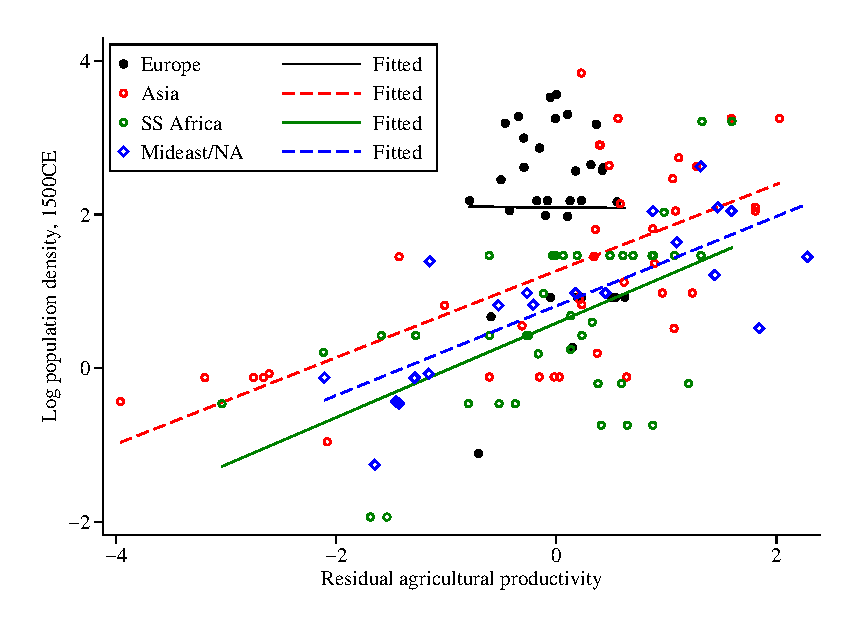
\includegraphics[width=1.0\textwidth]{fig_ag_regions.eps}
\end{center}
\vspace{-.5cm}\singlespacing {\footnotesize \textbf{Notes}: The figure replicates, by region, the regression from \citet{ashraf2010dynamics}, Table 2, column (4). We plot raw  population density in 1500CE against the residual variation in agricultural productivity, after controlling for (log) years since the Neolithic transition, (log) absolute latitude, the mean distance to a coast or river, and the percent of land less than 100 km from a coast or river. Agricultural productivity, from \citet{ashraf2010dynamics}, is the first principal component of the percent of arable land and a measure of cultivation suitability from \citet{ramankutty2002}. See appendix for lists of exact countries included in each region.
}
\end{figure}

\clearpage

\begin{figure}[!htb]
\begin{center}
\caption{Urbanization and Population Density, by Region, 1500CE}
\label{FIG_ag_urban}
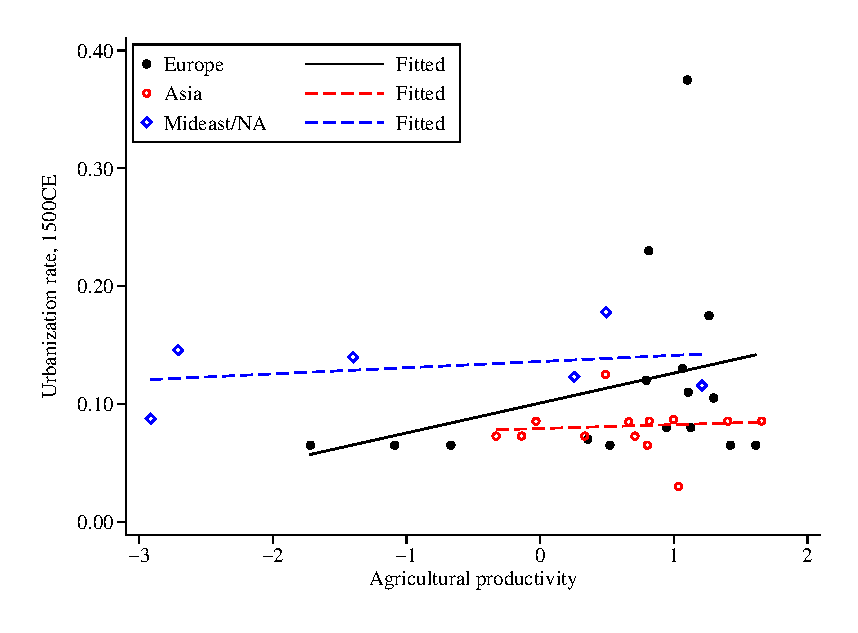
\includegraphics[width=1.0\textwidth]{fig_ag_urban.eps}
\end{center}
\end{figure}

\begin{figure}[!htb]
\begin{center}
\caption{Caloric Yield and Rural Density, by Major Crop, 2000CE}
\label{FIG_beta_crop}
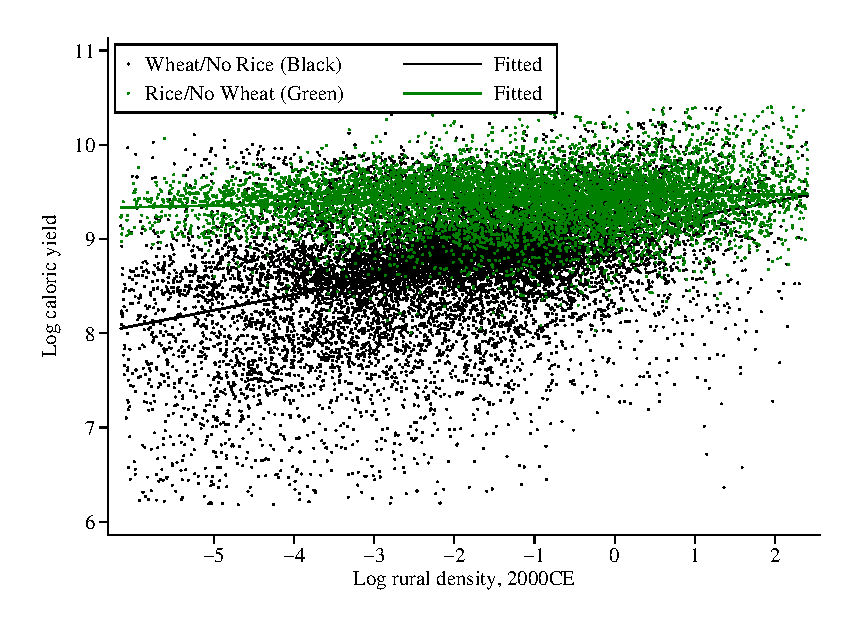
\includegraphics[width=1.0\textwidth]{fig_beta_crop.eps}
\end{center}
\vspace{-.5cm}\singlespacing {\footnotesize \textbf{Notes}: This figures shows the raw correlation of (log) caloric yield and (log) rural density for districts that are (a) suitable for wheat, but not for rice, and (b) suitable for rice but not for wheat. Rural population is from HYDE database \citep{hyde31}, and caloric yield is the author's calculations based on the data from \citet{galorozak2016}. The linear fits are from bivariate OLS regressions, without country fixed effects included.
}
\end{figure}


\clearpage
\begin{table}[!htb]
\begin{center}
\caption{Population Density and Land Productivity, by Region, 1500CE}
\label{TAB_ag_regions}
{\small
\begin{tabularx}{\textwidth}{lXXXXXX}
\midrule
\multicolumn{7}{l}{Dependent Variable: Log population density:} \\
 & \multicolumn{6}{c}{Region:} \\ \cmidrule{2-7}
 &        &      &       & Sub-      & North     & \\
 &        &      &       & Saharan   & Africa \& & \\
 & All & Europe  & Asia  & Africa    & Mideast   & Americas \\
 & (1) & (2) & (3) & (4) & (5) & (6) \\
\midrule
Log Land Productivity&       0.533&      -0.013&       0.558&       0.615&       0.583&       0.324\\
                    &     (0.059)&     (0.427)&     (0.062)&     (0.116)&     (0.070)&     (0.308)\\
\midrule
Observations        &         147&          33&          40&          39&          21&          25\\
Adjusted R-square   &        0.67&        0.39&        0.65&        0.71&        0.80&        0.46\\

\midrule
\end{tabularx}
}
\end{center}
\vspace{-.5cm}\singlespacing {\footnotesize \textbf{Notes}: Standard errors are robust, *** indicates significance at 1\%, ** at 5\%, and * at 10\%. Regression (1) includes continent fixed effects for Europe, Asia, and Africa; the Americas is the excluded category, and the North Africa/Mid-east category overlaps with Asia and Africa. See appendix for lists of exact countries included in each region. All regressions includes controls (log) years since the Neolithic transition, (log) absolute latitude, the mean distance to a coast or river, and the percent of land less than 100 km from a coast or river. The data is drawn directly from \citet{ashraf2010dynamics}, and column (1) replicates their result.
}
\end{table}

\clearpage
\begin{table}[!htb]
\begin{center}
\caption{Estimates of Malthusian Tightness, $\beta$, by Region, 2000CE}
\label{TAB_beta_region}
{\small
\begin{tabularx}{\textwidth}{lXXXXXX}
\midrule
\multicolumn{7}{l}{Dependent Variable: Log caloric yield ($A_{ic}$)} \\
 & \multicolumn{6}{c}{Region:} \\ \cmidrule{2-7}
 &        &      & Sub-        & South \&  & North     &  \\
 &        &      & Saharan     & Central   & Africa \& & North \\
 & Europe & Asia & Africa      & America   & Mideast   & America \\
 & (1) & (2) & (3) & (4) & (5) & (6) \\
\midrule
Log rural density   &       0.279&       0.157&       0.104&       0.213&       0.119&       0.203\\
                    &     (0.013)&     (0.010)&     (0.011)&     (0.015)&     (0.011)&     (0.042)\\
\midrule
p-value $\beta=0$   &       0.000&       0.000&       0.000&       0.000&       0.000&       0.000\\
p-value $\beta=\beta^{Eur}$&           .&       0.000&       0.000&       0.001&       0.000&       0.082\\
Countries           &          34&          24&          43&          18&          25&           2\\
Observations        &        7514&        6761&        3210&        2762&        9131&        2782\\
Adjusted R-square   &        0.30&        0.24&        0.26&        0.28&        0.18&        0.28\\

\midrule
\end{tabularx}
}
\end{center}
\vspace{-.5cm}\singlespacing {\footnotesize \textbf{Notes}: Standard errors are clustered at the country level, *** indicates significance at 1\%, ** at 5\%, and * at 10\%. All regressions include country fixed effects and a constant. See appendix for lists of exact countries included in each region. The coefficient estimate on rural population density indicates the value of $\beta$, see equation (\ref{EQ_regress}). Rural population is from HYDE database \citep{hyde31}, and caloric yield is the author's calculations based on the data from \citet{galorozak2016}. The p-value is from a hypothesis test that the estimated $\beta$ is equal to that estimated for Europe, $\beta^{Eur}$, and is obtained from an interaction term in a separate regression including both Europe and the given region, see equation (\ref{EQ_interaction}) and the text for details.
}
\end{table}


\clearpage
\begin{table}[!htb]
\begin{center}
\caption{Estimates of Malthusian Tightness, $\beta$, by Sub-regions, 2000CE}
\label{TAB_beta_subregion}
{\small
\begin{tabularx}{\textwidth}{lXXXXX}
\midrule
\multicolumn{6}{l}{Dependent Variable in both panels: Log caloric yield ($A_{ic}$)} \\ \\
\\
Panel A & \multicolumn{5}{c}{Sub-Region:} \\ \cmidrule{2-6}
 &          &         &             &  \multicolumn{2}{c}{Excl. China} \\ \cmidrule(lr){5-6}
 & North \& &         &              & South \&  & Central \&             \\
 & Western  & Eastern & Southern     & Southeast & West        \\
 & Europe   & Europe  & Europe       & Asia      & Asia      \\
 & (1) & (2) & (3) & (4) & (5) \\
\midrule
Log rural density   &       0.264&       0.292&       0.271&       0.148&       0.184\\
                    &     (0.033)&     (0.016)&     (0.021)&     (0.014)&     (0.015)\\
\midrule
p-value $\beta=0$   &       0.000&       0.000&       0.000&       0.000&       0.000\\
p-value $\beta=\beta^{NWEur}$&           .&       0.435&       0.847&       0.001&       0.028\\
Countries           &          16&           9&           9&          13&          18\\
Observations        &        1628&        4772&        1114&        3921&        2762\\
Adjusted R-square   &        0.21&        0.31&        0.26&        0.16&        0.18\\

\midrule
\\
Panel B & \multicolumn{5}{c}{Sub-Region:} \\ \cmidrule{2-6}
 &           &   &           &          &             \\
 & Temperate & Tropical  & Tropical & South    & North    \\
 & Americas  & Americas  & Africa   & Africa   & Africa     \\
\midrule
Log rural density   &       0.187&       0.119&       0.100&       0.130&       0.282\\
                    &     (0.039)&     (0.011)&     (0.011)&     (0.061)&     (0.019)\\
\midrule
p-value $\beta=0$   &       0.000&       0.000&       0.000&       0.033&       0.000\\
p-value $\beta=\beta^{NWEur}$&       0.137&       0.000&       0.000&       0.054&       0.630\\
Countries           &           5&          22&          39&           4&           5\\
Observations        &        3183&        8730&        3032&         178&        1147\\
Adjusted R-square   &        0.18&        0.10&        0.14&        0.19&        0.24\\

\midrule
\end{tabularx}
}
\end{center}
\vspace{-.5cm}\singlespacing {\footnotesize \textbf{Notes}: Standard errors are clustered at the country level, *** indicates significance at 1\%, ** at 5\%, and * at 10\%. All regressions include country fixed effects and a constant. See appendix for lists of exact countries included in each region. The coefficient estimate on rural population density indicates the value of $\beta$, see equation (\ref{EQ_regress}). Rural population is from HYDE database \citep{hyde31}, and caloric yield is the author's calculations based on the data from \citet{galorozak2016}. The p-value is from a hypothesis test that the estimated $\beta$ is equal to that estimated for Northwest Europe, $\beta^{NWEur}$, and is obtained from an interaction term in a separate regression including both Northwest Europe and the given region, see equation (\ref{EQ_interaction}) and the text for details.
}
\end{table}

\clearpage
\begin{table}[!htb]
\begin{center}
\caption{Estimates of Malthusian Tightness, $\beta$, China, 2000CE}
\label{TAB_beta_china}
{\small
\begin{tabularx}{\textwidth}{lXXXXXX}
\midrule
\multicolumn{7}{l}{Dependent Variable: Log caloric yield ($A_{ic}$)} \\
 & \multicolumn{3}{c}{Province level:} & \multicolumn{3}{c}{District level:} \\ \cmidrule(lr){2-4} \cmidrule(lr){5-7}
 & All& North & South & All   & North   & South \\
 & China & China  & China      & China    & China   & China \\
 & (1) & (2) & (3) & (4) & (5) & (6) \\
\midrule
Log rural density   &       0.509&       0.485&       0.113&       0.461&       0.509&       0.091\\
                    &     (0.065)&     (0.057)&     (0.080)&     (0.042)&     (0.044)&     (0.020)\\
\midrule
p-value $\beta=\beta^{North}$&            &            &       0.001&            &            &       0.000\\
Observations        &          26&          12&          14&         294&         137&         157\\
Adjusted R-square   &        0.69&        0.68&        0.07&        0.36&        0.32&        0.17\\

\midrule
\end{tabularx}
}
\end{center}
\vspace{-.5cm}\singlespacing {\footnotesize \textbf{Notes}: Standard errors are clustered at the country level, *** indicates significance at 1\%, ** at 5\%, and * at 10\%. All regressions include country fixed effects and a constant. See appendix for lists of exact countries included in each region. The coefficient estimate on rural population density indicates the value of $\beta$, see equation (\ref{EQ_regress}). Rural population is from HYDE database \citep{hyde31}, and caloric yield is the author's calculations based on the data from \citet{galorozak2016}. The p-value is from a hypothesis test that the estimated $\beta$ is equal to that estimated for North China, $\beta^{North}$, and is obtained from an interaction term in a separate regression including both North and South China, see equation (\ref{EQ_interaction}) and the text for details.
}
\end{table}

\clearpage
\begin{table}[!htb]
\begin{center}
\caption{Estimates of Malthusian Tightness, $\beta$, by Crop Suitability, 2000CE}
\label{TAB_beta_crops}
{\footnotesize
\begin{tabularx}{\textwidth}{lXXXXXX}
\midrule
\multicolumn{7}{l}{Dependent Variable in all panels: Log caloric yield ($A_{ic}$)} \\ \\
\multicolumn{7}{l}{Panel A: Wheat and rice} \\
 & \multicolumn{6}{c}{Inclusion by crop suitability:} \\ \cmidrule(lr){2-7}
 & \multicolumn{4}{c}{Entire world:} & \multicolumn{2}{c}{Ex. Americas:}\\ \cmidrule(lr){2-5} \cmidrule(lr){6-7} 
 & Wheat$>$0& Wheat=0 &         &        & Wheat$>$0   & Wheat=0   \\
 & Rice=0 & Rice$>$0  & Wheat$>$0 & Rice$>$0 & Rice=0    & Rice$>$0   \\
 & (1) & (2) & (3) & (4) & (5) & (6) \\
\midrule
rurd_reg            &       0.227&       0.138\\
                    &     (0.024)&     (0.021)\\
\midrule
p-value $\beta=0$   &       0.000&       0.000\\
p-value $\beta=\beta^{Wheat}$&            &    .0049448\\
Countries           &         106&          74\\
Observations        &    12627.00&    20423.00\\
Adjusted R-square   &        0.21&        0.19\\

\midrule
\\
\multicolumn{7}{l}{Panel B: Tropical crops} \\
                   & \multicolumn{6}{c}{Inclusion is wheat suitability = 0, but:} \\ \cmidrule(lr){2-7}
                   &            &              &          &   Pearl       &  Sweet      & \\
& Cassava$>$0 & Cowpeas$>$0  & Maize$>$0 & Millet$>$0 & Potato$>$0 & Yams$>$0   \\
\midrule
Log rural density   &       0.140&       0.144&       0.143&       0.154&       0.144&       0.140\\
                    &     (0.021)&     (0.020)&     (0.020)&     (0.019)&     (0.020)&     (0.020)\\
\midrule
p-value $\beta=0$   &       0.000&       0.000&       0.000&       0.000&       0.000&       0.000\\
Countries           &          74&          80&          78&          72&          77&          78\\
Observations        &        8052&        8312&        8377&        6590&        8354&        8269\\
Adjusted R-square   &        0.13&        0.13&        0.13&        0.13&        0.13&        0.12\\

\midrule
\\
\multicolumn{7}{l}{Panel C: Temperate crops} \\
                   & \multicolumn{6}{c}{Inclusion is rice suitability = 0, but:} \\ \cmidrule(lr){2-7}
                   &            & Buck-        &          &          &         & White \\
                   & Barley$>$0 & wheat$>$0  & Oats$>$0 & Flax$>$0 & Rye$>$0 & Potato$>$0   \\
\midrule
Log rural density   &       0.227&       0.228&       0.234&       0.228&       0.235&       0.227\\
                    &     (0.024)&     (0.025)&     (0.025)&     (0.025)&     (0.025)&     (0.023)\\
\midrule
p-value $\beta=0$   &       0.000&       0.000&       0.000&       0.000&       0.000&       0.000\\
Countries           &         106&          76&          72&          74&          72&         105\\
Observations        &       12627&       11162&       11089&       11035&       11106&       12494\\
Adjusted R-square   &        0.21&        0.23&        0.23&        0.23&        0.23&        0.22\\

\midrule
\end{tabularx}
}
\end{center}
\vspace{-.5cm}\singlespacing {\footnotesize \textbf{Notes}: Standard errors are clustered at the country level, *** indicates significance at 1\%, ** at 5\%, and * at 10\%. All regressions include country fixed effects and a constant. The coefficient estimate on rural population density indicates the value of $\beta$, see equation (\ref{EQ_regress}). Rural population is from HYDE database \citep{hyde31}, and caloric yield is the author's calculations based on the data from \citet{galorozak2016}. Inclusion of sub-national units in the regression is based on crop suitability indices from \citet{gaez}, which range from 0 to 100, and are calculated by the author's for each sub-national unit. See text for details.
}
\end{table}


\end{document}